\chapter{ANOVA}
One-way ANOVA is a common procedure in statistics, and is related to the
simpler idea of a t-test. In this chapter we will look at the same questions
but will answer them using a Bayesian model instead of a classical statistical
test.

\section{A T-Test}
We will look at a simple example first, and then a more complex one.
The first example is based on one given in a 1976 article by physicist E. T. Jaynes,
called ``Confidence Intervals vs. Bayesian Intervals''. This is a very strongly
worded paper and might be an interesting read for
those who are interested in the battle between frequentist and Bayesian statistics
when the latter was making its comeback in the second half of the 20th century.
It's also where I got the crazy confidence interval example from.

Two manufacturers, $A$ and $B$, both make ``widgets'', and we are interested
in figuring out which manufacturer makes the best widgets (on average), as
measured by their lifetime. To determine this, we obtain 9 widgets from
manufacturer $A$ and 4 widgets from manufacturer $B$. The results for the
lifetimes are given below:
\begin{eqnarray}
y_A = \{ \}
\end{eqnarray}
Classically, this could be solved by using a $t$-test.

The underlying assumption of a $t$-test is that the data are normally
distributed around the mean values for each group. If we call the group 1
data points $\{y^1_1, y^1_2, ..., y^1_{N_1}\}$ and the group 2 data points
$\{y^2_1, y^2_2, ..., y^2_{N_1}\}$, then the likelihood is:
\begin{eqnarray}
y^1_i &\sim& \mathcal{N}\left(\mu_1, \sigma^2\right)\\
y^2_i &\sim& \mathcal{N}\left(\mu_2, \sigma^2\right)\\
\end{eqnarray}
Where all the data points are independent given the parameters. Note the assumption that
the two groups have the same standard deviation $\sigma$. This is a popular
assumption in this kind of analysis but it is not necessarily well justified!
We will build our Bayesian models using this assumption, but it is not that
difficult to relax it if you want to (just include multiple $\sigma$ parameters
in similar ways to how we will include the multiple $\mu$ parameters).

We will study three variations on the t-test. They all have the same likelihood
as given above,
but will different priors for the unknown parameters $\mu_1$, $\mu_2$, and
$\sigma$.
We will be able to see that the choice of prior does
influence the results (of course), but in ways that make sense. Which of these
models is more appropriate in a practical situation would depend on the exact
situation: there is no ``one size fits all'' model.

\subsection{Naive Model}

\begin{framed}
\begin{verbatim}
# Actually allow mu1=mu2
model
{
    # Log-uniform prior for the s.d.
    log_sigma ~ dunif(-5, 5)
    sigma <- exp(log_sigma)

    # First mean
    mu1 ~ dunif(-1000, 1000)

    # Prior on second mean
    mu2 ~ dunif(-1000, 1000)

    # Sampling distribution/likelihood
    for(i in 1:N1)
    {
        y1[i] ~ dnorm(mu1, pow(sigma, -2))
    }
    for(i in 1:N2)
    {
        y2[i] ~ dnorm(mu2, pow(sigma, -2))
    }

}
\end{verbatim}
\end{framed}

\subsection{Model that allows exact equality}

\begin{framed}
\begin{verbatim}
# Actually allow mu1=mu2
model
{
    # Log-uniform prior for the s.d.
    log_sigma ~ dunif(-5, 5)
    sigma <- exp(log_sigma)

    # First mean
    mu1 ~ dunif(-1000, 1000)

    # Prior on second mean
    difference ~ dt(0., pow(5., -2), 1.)
    flag ~ dunif(0., 1.)
    mu2 <- mu1 + step(flag - 0.5)*difference

    # Sampling distribution/likelihood
    for(i in 1:N1)
    {
        y1[i] ~ dnorm(mu1, pow(sigma, -2))
    }
    for(i in 1:N2)
    {
        y2[i] ~ dnorm(mu2, pow(sigma, -2))
    }

}
\end{verbatim}
\end{framed}

The results of the three different models are shown below:
\begin{figure}
\begin{center}
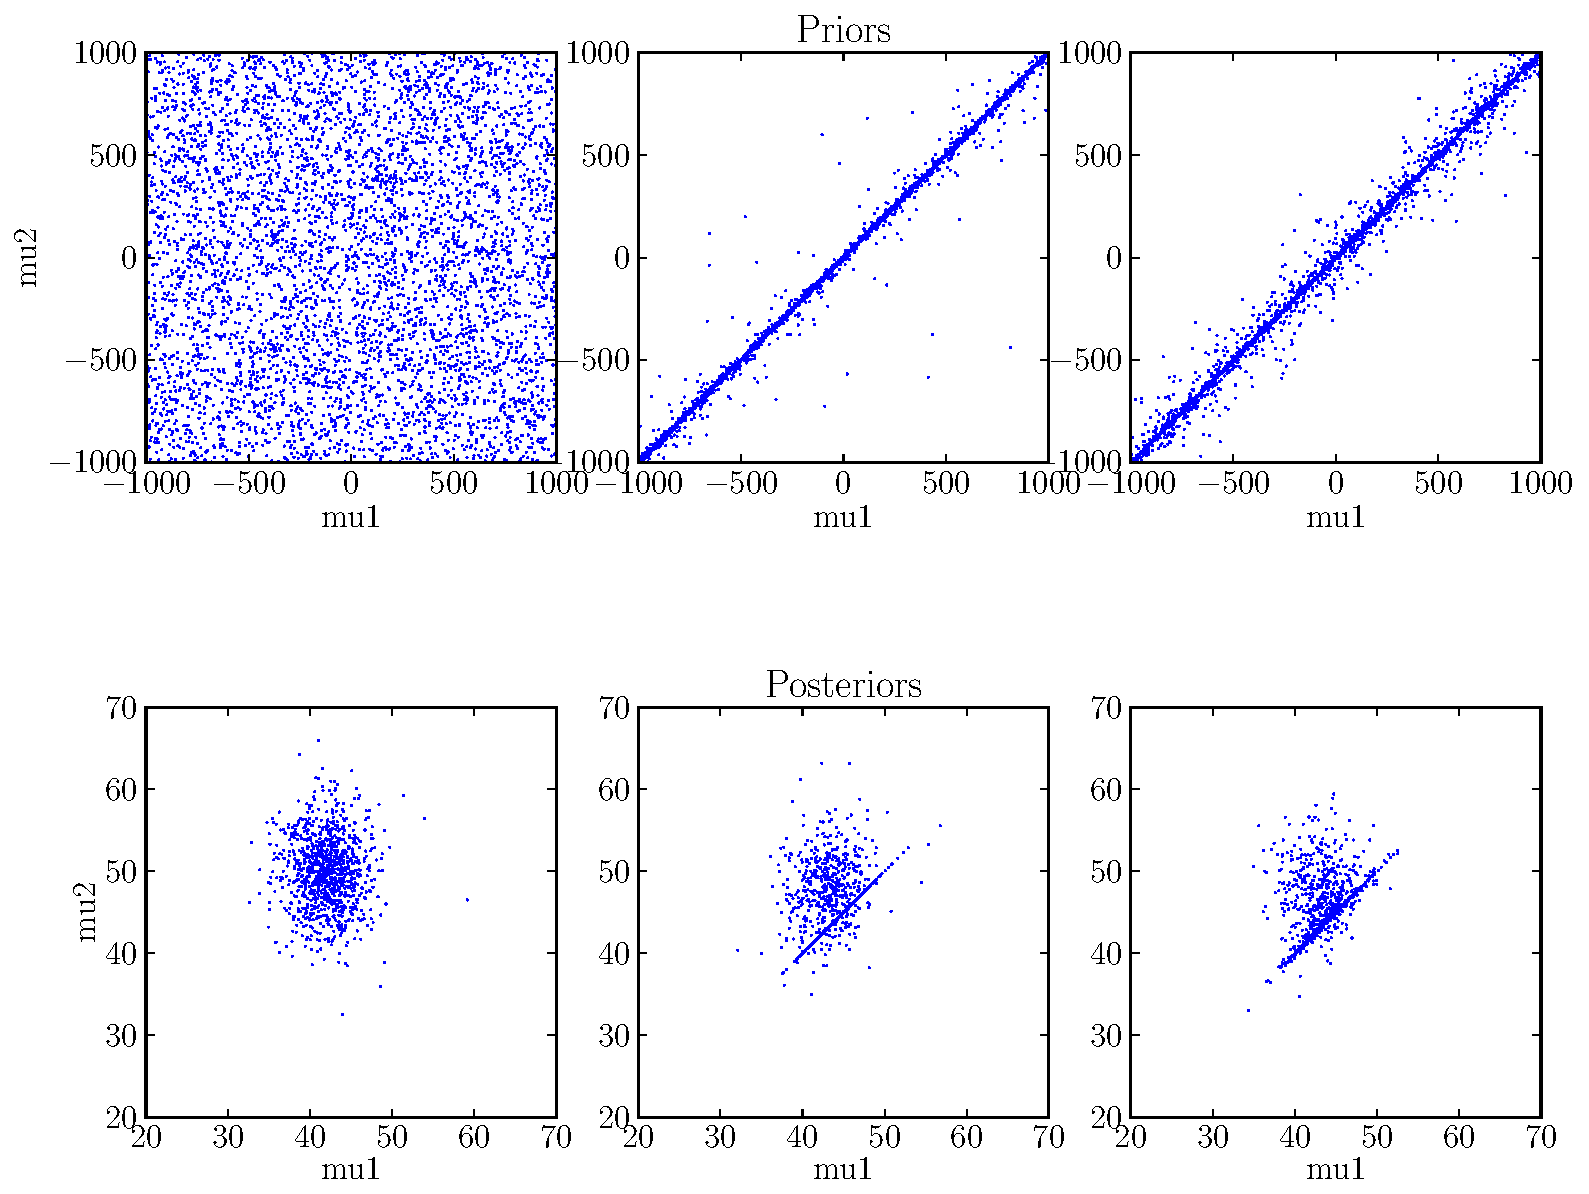
\includegraphics[scale=0.8]{Figures/ttest.pdf}
\end{center}
\end{figure}


\subsection{Hierarchical Model}


The main advantage of this model is that it generalises to more than two groups
in a very straightforward way.
\begin{framed}
\begin{verbatim}
model
{
    # Log-uniform prior for the s.d.
    log_sigma ~ dunif(-5, 5)
    sigma <- exp(log_sigma)

    # Hierarchical prior for the means
    # Hyperparameters
    grand_mean ~ dunif(-1000, 1000)
    log_diversity ~ dunif(-5., 5.)
    diversity <- exp(log_diversity)

    # Parameters
    mu1 ~ dnorm(grand_mean, pow(diversity, -2))
    mu2 ~ dnorm(grand_mean, pow(diversity, -2))

    # Sampling distribution/likelihood
    for(i in 1:N1)
    {
        y1[i] ~ dnorm(mu1, pow(sigma, -2))
    }
    for(i in 1:N2)
    {
        y2[i] ~ dnorm(mu2, pow(sigma, -2))
    }
}

\end{verbatim}
\end{framed}



\section{One Way Anova}
One-way ANOVA can be considered as a generalisation of a t-test to more than
two groups. The question is usually phrased as a test of the hypothesis that
the group means are the same, versus the alternative that there is some difference.
As we saw in the Bayesian ``t-test'', it is possible (using clever tricks) to
make a model that has some prior probability that the group means are equal.
However, this gets more tricky with multiple groups. Therefore we will build our
one-way ANOVA model in a similar way to the ``hierarchical model'' version of the
t-test model.

*real example*



